\documentclass[12pt, letterpaper]{article}

% -------------------------
% PAQUETES
% -------------------------
\usepackage[utf8]{inputenc}
\usepackage[T1]{fontenc}
\usepackage[spanish]{babel}
\usepackage{geometry}
\usepackage{graphicx}
\usepackage{float}
\usepackage{booktabs}
\usepackage{longtable}
\usepackage{array}
\usepackage{amsmath}
\usepackage{amssymb}
\usepackage{xcolor}
\usepackage{caption}
\usepackage{subcaption}
\usepackage{fancyhdr}
\usepackage{hyperref}
\usepackage{enumitem}
\usepackage{tocbibind}
% -------------------------
% CONFIGURACIÓN DE PÁGINA
% -------------------------
\geometry{
    top=2.5cm,
    bottom=2.5cm,
    left=2.5cm,
    right=2.5cm
}

\hypersetup{
    colorlinks=true,
    linkcolor=black,
    urlcolor=blue,
    citecolor=black
}

\setlength{\parskip}{6pt}
\setlength{\parindent}{0pt}

\pagestyle{fancy}
\fancyhf{}
\fancyhead[L]{CE1111 -- Análisis Numérico}
\fancyhead[R]{Reconocimiento facial}
\fancyfoot[C]{\thepage}
\setlength{\headheight}{15pt}

% -------------------------
% DATOS DEL INFORME
% -------------------------
\newcommand{\universidad}{Instituto Tecnológico de Costa Rica}
\newcommand{\curso}{CE1111 -- Análisis Numérico para Ingeniería}
\newcommand{\titulo}{Reconocimiento facial mediante valores y vectores propios}
\newcommand{\estudiantes}{%
    Joaquin Ignacio Ramirez Sequeira\\
    Joseph Stif Piedra Montero%
}
\newcommand{\profesor}{Juan Pablo Soto Quirós}
\newcommand{\semestre}{Semestre II, 2026}
\newcommand{\fecha}{\today}

\begin{document}

% =================================================
% PORTADA
% =================================================
\begin{titlepage}
    \centering
    \vspace*{1cm}
    {\Large\textbf{\universidad}\par}
    \vspace{1.5cm}
    % \includegraphics[width=0.22\textwidth]{logo.png}
    \vspace{1cm}
    {\large\curso\par}
    \vspace{2cm}
    {\LARGE\bfseries \titulo\par}
    \vspace{0.8cm}
    {\large Informe de resultados\par}
    \vspace{2cm}
    \begin{flushleft}
        \textbf{Estudiantes:}\\
        \estudiantes
        \vspace{0.6cm}

        \textbf{Docente:}\\
        \profesor
        \vspace{0.6cm}

        \textbf{Periodo académico:}\\
        \semestre
    \end{flushleft}
    \vfill
    {\large \fecha\par}
\end{titlepage}

% =================================================
% CONTENIDO
% =================================================
\tableofcontents
\newpage

% =================================================
\section{Introducción}
% =================================================

En este informe se presentan los resultados obtenidos al aplicar
el método de reconocimiento facial basado en valores y vectores
propios (eigenfaces) sobre la base de datos \textit{AT\&T Database
of Faces}. Se emplearon 360 fotografías para entrenamiento
(nueve por cada una de las 40 personas) y 40 fotografías para
prueba (la décima fotografía de cada persona).

El procedimiento sigue los pasos del documento \textit{rec\_facial.pdf}.
Primero se preprocesan las imágenes y se vectorizan. Luego se calcula el
rostro promedio y se construye la matriz centrada $A$. Después se obtienen
los valores y vectores propios de $G = AA^{T}$ con el método QR implementado
desde cero. Con eso se elige el número de caras base $k$. Al final se
proyectan las imágenes de prueba sobre el subespacio facial y se clasifican
por vecino más cercano.

% =================================================
\section{Justificación del método numérico}
% =================================================

La elección se basa en los resultados de la Parte II. Allí se compararon
QR y Jacobi sobre una matriz tridiagonal simétrica de $200 \times 200$ con
tolerancia $10^{-8}$ y un máximo de $10^{4}$ iteraciones. Los resultados fueron:

\begin{itemize}
    \item \textbf{QR} alcanzó la tolerancia en aproximadamente $10^{3}$
    iteraciones. Su error final fue del orden de $10^{-7}$.

    \item \textbf{Jacobi} agotó las iteraciones sin alcanzar la tolerancia.
    Su error final quedó en $5 \times 10^{-6}$.
\end{itemize}

QR fue el único método que convergió dentro del máximo de iteraciones
permitido. Por eso se usó para calcular las eigenfaces en esta Parte III.

% =================================================
\section{Rostro promedio y caras base}
% =================================================

\subsection{Rostro promedio}

El rostro promedio $\bar{f}$ se calcula exclusivamente a partir
de las 360 fotografías del conjunto de entrenamiento:
\[
    \bar{f} = \frac{1}{360} \sum_{i=1}^{360} f_i
\]
donde cada $f_i \in \mathbb{R}^{2576}$ es una fotografía
vectorizada por columnas. Esta imagen representa las
características promedio del conjunto.

\begin{figure}[H]
    \centering
    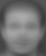
\includegraphics[width=0.32\textwidth]{resultados_parte3/rostro_medio.png}
    \caption{Rostro promedio del conjunto de entrenamiento.}
    \label{fig:rostro-promedio}
\end{figure}

\subsection{Primeras seis caras base}

Las caras base son los vectores propios $\mathbf{u}_1, \dots, \mathbf{u}_k$
de la matriz $G = AA^{T}$ asociados a los $k$ valores propios
más grandes. Cada cara base tiene 2576 componentes y puede
visualizarse como una imagen de $56 \times 46$ píxeles. No
corresponden a personas concretas, sino a patrones de variación
del conjunto de entrenamiento. Las primeras seis se muestran en
la Figura~\ref{fig:caras-base}.

\begin{figure}[H]
    \centering

    % --- Fila 1: caras base 1, 2, 3 ---
    \begin{subfigure}[b]{0.20\textwidth}
        \centering
        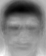
\includegraphics[width=\textwidth]{resultados_parte3/eigenface_1.png}
        \caption*{Cara base 1}
    \end{subfigure}
    \hfill
    \begin{subfigure}[b]{0.20\textwidth}
        \centering
        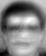
\includegraphics[width=\textwidth]{resultados_parte3/eigenface_2.png}
        \caption*{Cara base 2}
    \end{subfigure}
    \hfill
    \begin{subfigure}[b]{0.20\textwidth}
        \centering
        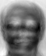
\includegraphics[width=\textwidth]{resultados_parte3/eigenface_3.png}
        \caption*{Cara base 3}
    \end{subfigure}

    \vspace{0.3cm}

    % --- Fila 2: caras base 4, 5, 6 ---
    \begin{subfigure}[b]{0.20\textwidth}
        \centering
        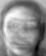
\includegraphics[width=\textwidth]{resultados_parte3/eigenface_4.png}
        \caption*{Cara base 4}
    \end{subfigure}
    \hfill
    \begin{subfigure}[b]{0.20\textwidth}
        \centering
        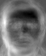
\includegraphics[width=\textwidth]{resultados_parte3/eigenface_5.png}
        \caption*{Cara base 5}
    \end{subfigure}
    \hfill
    \begin{subfigure}[b]{0.20\textwidth}
        \centering
        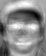
\includegraphics[width=\textwidth]{resultados_parte3/eigenface_6.png}
        \caption*{Cara base 6}
    \end{subfigure}

    \caption{Primeras seis caras base obtenidas a partir del
    conjunto de entrenamiento. Representan patrones de variación,
    no personas concretas.}
    \label{fig:caras-base}
\end{figure}
% =================================================
\section{Parámetros y variación conservada}
% =================================================

Los valores propios de $G = AA^{T}$ se ordenaron de mayor a menor
y se descartaron aquellos numéricamente nulos, conservando
únicamente los que satisfacen $\lambda_j > 10^{-10}\,\lambda_1$.
Los resultados obtenidos fueron:

\begin{itemize}
    \item \textbf{Valores propios retenidos ($r$):} $r = 359$.
    \item \textbf{Caras base seleccionadas ($k$):} $k = 129$.
    \item \textbf{Proporción de variación conservada:} $95.01\%$.
\end{itemize}

La proporción de variación conservada se calcula mediante
\[
    V_k = \frac{\displaystyle\sum_{i=1}^{k}\lambda_i}
               {\displaystyle\sum_{i=1}^{r}\lambda_i} \times 100\%,
\]
donde $\lambda_i$ representa el $i$-ésimo valor propio. Con
$k = 129$ se conserva el $95.01\%$ de la variabilidad total.
La Figura~\ref{fig:variacion} muestra la variación acumulada en
función del número de caras base retenidas.

\begin{figure}[H]
    \centering
    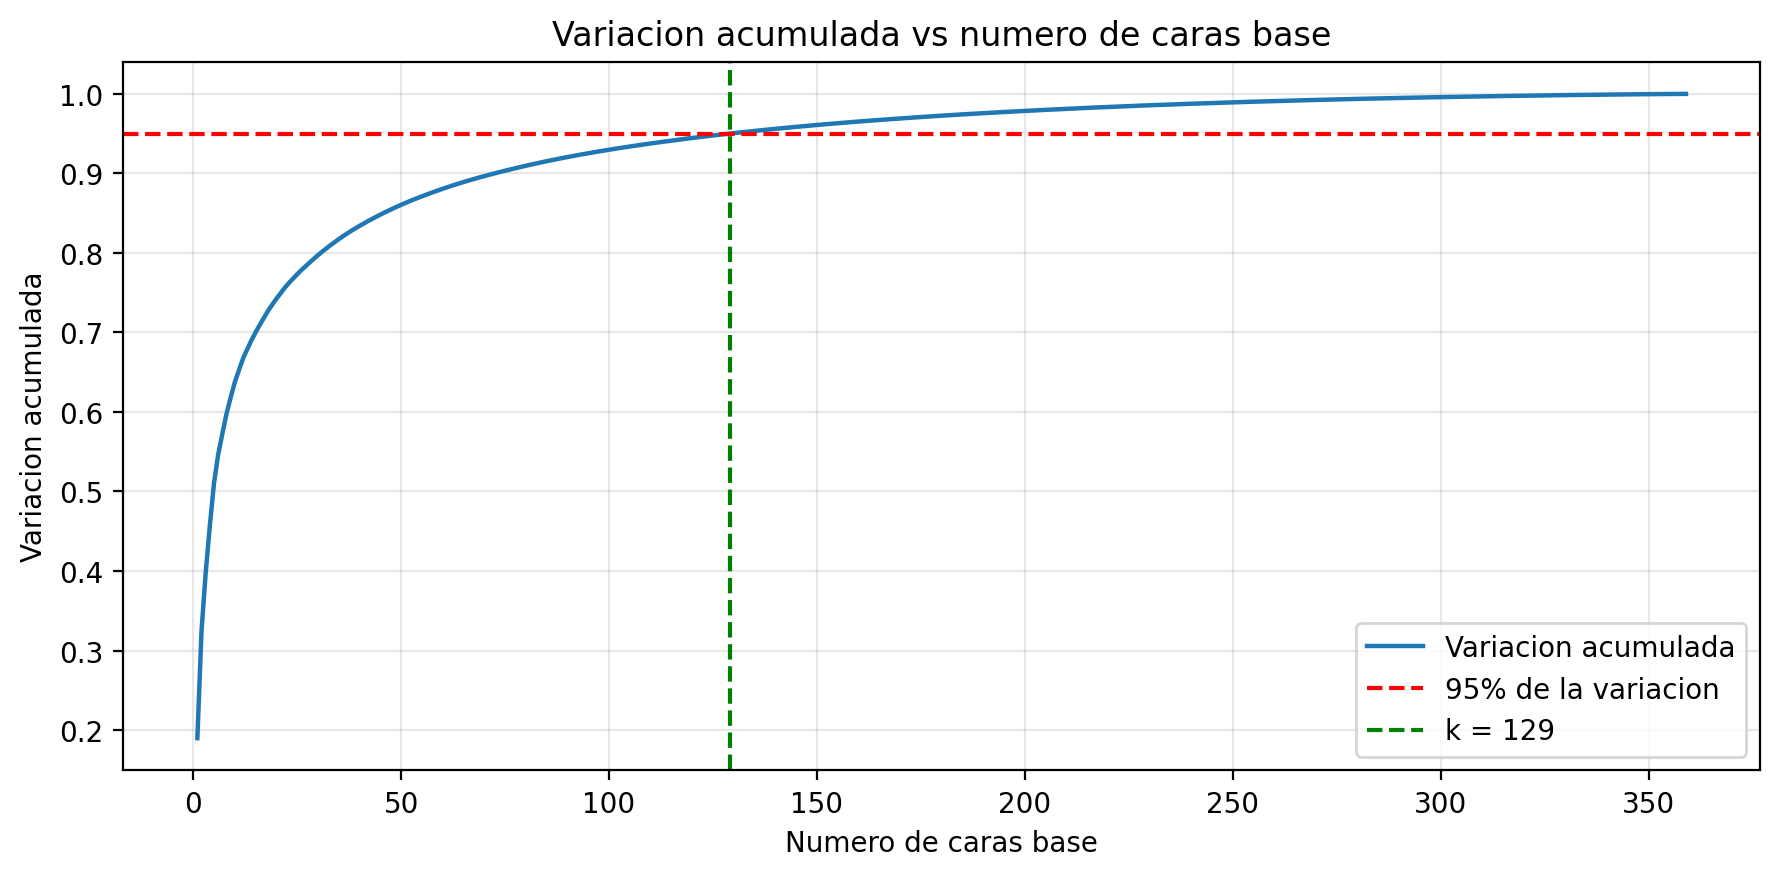
\includegraphics[width=0.85\textwidth]{resultados_parte3/variacion_acumulada.png}
    \caption{Variación acumulada en función del número de caras
    base. El corte en $k = 129$ conserva el $95.01\%$ de la
    variación total.}
    \label{fig:variacion}
\end{figure}

% =================================================
\section{Predicciones de las fotografías de prueba}
% =================================================

La Tabla~\ref{tab:predicciones} presenta las predicciones
obtenidas para las 40 fotografías de prueba. Para cada fotografía
se indica la identidad real, la identidad predicha y si la
identificación fue correcta. La identidad predicha corresponde
a la etiqueta de la imagen de entrenamiento más cercana en el
subespacio de $k = 129$ caras base, según distancia euclidiana.

\begin{longtable}{c c c c c}
    \caption{Predicciones para las 40 fotografías de prueba.}
    \label{tab:predicciones}\\
    \toprule
    \textbf{N.º} & \textbf{Foto} & \textbf{Real} &
    \textbf{Predicha} & \textbf{Resultado} \\
    \midrule
    \endfirsthead
    \toprule
    \textbf{N.º} & \textbf{Foto} & \textbf{Real} &
    \textbf{Predicha} & \textbf{Resultado} \\
    \midrule
    \endhead
    \bottomrule
    \endfoot
    1  & s1/10.png  & 1  & 1  & Correcta \\
    2  & s2/10.png  & 2  & 2  & Correcta \\
    3  & s3/10.png  & 3  & 3  & Correcta \\
    4  & s4/10.png  & 4  & 4  & Correcta \\
    5  & s5/10.png  & 5  & 40 & \textcolor{red}{Incorrecta} \\
    6  & s6/10.png  & 6  & 6  & Correcta \\
    7  & s7/10.png  & 7  & 7  & Correcta \\
    8  & s8/10.png  & 8  & 8  & Correcta \\
    9  & s9/10.png  & 9  & 9  & Correcta \\
    10 & s10/10.png & 10 & 38 & \textcolor{red}{Incorrecta} \\
    11 & s11/10.png & 11 & 11 & Correcta \\
    12 & s12/10.png & 12 & 12 & Correcta \\
    13 & s13/10.png & 13 & 13 & Correcta \\
    14 & s14/10.png & 14 & 14 & Correcta \\
    15 & s15/10.png & 15 & 15 & Correcta \\
    16 & s16/10.png & 16 & 16 & Correcta \\
    17 & s17/10.png & 17 & 17 & Correcta \\
    18 & s18/10.png & 18 & 18 & Correcta \\
    19 & s19/10.png & 19 & 19 & Correcta \\
    20 & s20/10.png & 20 & 20 & Correcta \\
    21 & s21/10.png & 21 & 21 & Correcta \\
    22 & s22/10.png & 22 & 22 & Correcta \\
    23 & s23/10.png & 23 & 23 & Correcta \\
    24 & s24/10.png & 24 & 24 & Correcta \\
    25 & s25/10.png & 25 & 25 & Correcta \\
    26 & s26/10.png & 26 & 26 & Correcta \\
    27 & s27/10.png & 27 & 27 & Correcta \\
    28 & s28/10.png & 28 & 28 & Correcta \\
    29 & s29/10.png & 29 & 29 & Correcta \\
    30 & s30/10.png & 30 & 30 & Correcta \\
    31 & s31/10.png & 31 & 31 & Correcta \\
    32 & s32/10.png & 32 & 32 & Correcta \\
    33 & s33/10.png & 33 & 33 & Correcta \\
    34 & s34/10.png & 34 & 34 & Correcta \\
    35 & s35/10.png & 35 & 35 & Correcta \\
    36 & s36/10.png & 36 & 36 & Correcta \\
    37 & s37/10.png & 37 & 37 & Correcta \\
    38 & s38/10.png & 38 & 38 & Correcta \\
    39 & s39/10.png & 39 & 39 & Correcta \\
    40 & s40/10.png & 40 & 40 & Correcta \\
\end{longtable}

% =================================================
\section{Exactitud del reconocimiento}
% =================================================

De las 40 fotografías de prueba, se obtuvieron los siguientes
resultados:

\begin{itemize}
    \item \textbf{Identificaciones correctas:} 38 de 40.
    \item \textbf{Identificaciones incorrectas:} 2.
    \item \textbf{Exactitud obtenida:} $95.00\%$.
\end{itemize}

La exactitud se calcula como:
\[
    \text{Exactitud} =
    \frac{\text{Identificaciones correctas}}
         {\text{Total de fotografías de prueba}} \times 100\%.
\]
Sustituyendo los resultados:
\[
    \text{Exactitud} = \frac{38}{40} \times 100\% = 95.00\%.
\]
% =================================================
\section{Comparación de fotografías}
% =================================================

Para cada una de las 40 personas se compara la fotografía de
prueba con la fotografía de entrenamiento más cercana encontrada
por el procedimiento. Se presentan a continuación cuatro casos
representativos: dos identificaciones correctas y las dos
identificaciones incorrectas.

\begin{figure}[H]
    \centering

    % ============ Fila 1 ============
    % Par 1: Persona 1 (correcta)
    \begin{subfigure}[b]{0.20\textwidth}
        \centering
        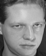
\includegraphics[width=\textwidth]{dataset_att/s1/10.png}
        \caption*{Prueba s1/10}
    \end{subfigure}
    \hspace{0.02\textwidth}
    \begin{subfigure}[b]{0.20\textwidth}
        \centering
        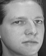
\includegraphics[width=\textwidth]{dataset_att/s1/5.png}
        \caption*{Vecino s1/5}
    \end{subfigure}
    \hspace{0.06\textwidth}    % separación entre pares
    % Par 2: Persona 33 (correcta)
    \begin{subfigure}[b]{0.20\textwidth}
        \centering
        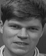
\includegraphics[width=\textwidth]{dataset_att/s33/10.png}
        \caption*{Prueba s33/10}
    \end{subfigure}
    \hspace{0.02\textwidth}
    \begin{subfigure}[b]{0.20\textwidth}
        \centering
        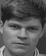
\includegraphics[width=\textwidth]{dataset_att/s33/2.png}
        \caption*{Vecino s33/2}
    \end{subfigure}

    \vspace{0.6cm}

    % ============ Fila 2 ============
    % Par 3: Persona 5 (incorrecta)
    \begin{subfigure}[b]{0.20\textwidth}
        \centering
        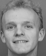
\includegraphics[width=\textwidth]{dataset_att/s5/10.png}
        \caption*{Prueba s5/10}
    \end{subfigure}
    \hspace{0.02\textwidth}
    \begin{subfigure}[b]{0.20\textwidth}
        \centering
        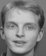
\includegraphics[width=\textwidth]{dataset_att/s40/5.png}
        \caption*{Vecino s40/5}
    \end{subfigure}
    \hspace{0.06\textwidth}    % separación entre pares
    % Par 4: Persona 10 (incorrecta)
    \begin{subfigure}[b]{0.20\textwidth}
        \centering
        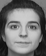
\includegraphics[width=\textwidth]{dataset_att/s10/10.png}
        \caption*{Prueba s10/10}
    \end{subfigure}
    \hspace{0.02\textwidth}
    \begin{subfigure}[b]{0.20\textwidth}
        \centering
        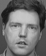
\includegraphics[width=\textwidth]{dataset_att/s38/4.png}
        \caption*{Vecino s38/4}
    \end{subfigure}

    \caption{Comparaciones representativas. Fila superior: dos
    identificaciones correctas (personas 1 y 33). Fila inferior:
    las dos identificaciones incorrectas (persona 5 confundida
    con la 40; persona 10 confundida con la 38).}
    \label{fig:comparaciones}
\end{figure}
% =================================================
\section{Análisis de confusiones e identificaciones incorrectas}
% =================================================

De las 40 fotografías de prueba se identificaron correctamente
38 y 2 se confundieron con otras personas.

\begin{itemize}
    \item \textbf{Persona 5} $\to$ identificada como
    \textbf{persona 40}. La fotografía \texttt{s5/10.png} quedó
    a distancia $4{,}2016$ de la imagen \texttt{s40/5.png}. Es
    una distancia moderada. La foto está lejos del resto de
    imágenes de la persona 5 pero más cerca de la persona 40.

    \item \textbf{Persona 10} $\to$ identificada como
    \textbf{persona 38}. La fotografía \texttt{s10/10.png} quedó
    a distancia $6{,}6093$ de \texttt{s38/4.png}. Es la distancia
    más grande de las 40 pruebas. Esto indica que la foto cae
    más lejos del subespacio facial que las demás.
\end{itemize}

Las causas posibles de estas confusiones son:

\begin{itemize}
    \item \textbf{Iluminación y pose.} Las fotos del conjunto
    AT\&T varían en iluminación y orientación. Cuando la foto de
    prueba se ve muy distinta al resto de fotos de la misma
    persona su proyección queda lejos del grupo correcto.

    \item \textbf{Parecido entre personas.} Algunos rasgos como
    la forma del rostro los lentes o la barba pueden acercar a
    dos personas distintas dentro del subespacio facial.

    \item \textbf{Pérdida de información.} Al retener solo
    $k = 129$ componentes principales se descartan variaciones
    finas que podrían separar a personas parecidas. La
    información descartada es el $4{,}99\%$ de la variabilidad.
\end{itemize}

% =================================================
\section{Papel de los valores y vectores propios}
% =================================================

El método de eigenfaces se basa en la descomposición espectral
de la matriz $G = AA^{T}$ de tamaño $2576 \times 2576$ donde
$A$ es la matriz de imágenes centradas. Los puntos clave son:

\begin{itemize}
    \item \textbf{Valores propios $\lambda_j$.} Miden cuánta
    variación de las imágenes centradas explica cada dirección
    principal. Los primeros concentran la mayor parte de la
    variabilidad. Los últimos aportan cada vez menos información
    útil y capturan sobre todo detalles finos y ruido de
    iluminación.

    \item \textbf{Vectores propios $\mathbf{u}_j$ (caras base).}
    Son las direcciones principales del subespacio facial. Cada
    uno tiene 2576 componentes y se puede ver como una imagen de
    $56 \times 46$. No representan personas concretas sino
    patrones de variación compartidos por el conjunto de
    entrenamiento.

    \item \textbf{Reducción de dimensión.} Se retuvieron
    $k = 129$ caras base que conservan el $95{,}01\%$ de la
    variación total. Cada fotografía pasa de representarse con
    $2576$ píxeles a representarse con $129$ coordenadas. La
    dimensión se reduce aproximadamente 20 veces.

    \item \textbf{Clasificación por vecino más cercano.} La
    identificación se hace proyectando la foto de prueba sobre
    las $k$ caras base y comparando sus coordenadas con las de
    las 360 imágenes de entrenamiento usando distancia euclidiana.
    Se asigna la etiqueta del vecino más cercano.

    \item \textbf{Eliminación de ruido.} Además de acelerar el
    reconocimiento la reducción de dimensión descarta variaciones
    menores como iluminación global o sombras suaves. Esto hace
    al método más robusto ante pequeñas diferencias entre fotos.
\end{itemize}

Se verificó numéricamente la ortogonalidad de las caras base
retenidas:
\[
    \|U_k^{T} U_k - I_k\|_F \approx 7{,}25 \times 10^{-14}.
\]
El resultado confirma que las $k$ caras base son ortonormales
entre sí como corresponde a una matriz simétrica.

% =================================================
\section{Conclusiones}
% =================================================

\begin{itemize}
    \item El método QR implementado desde cero calculó los
    valores y vectores propios de $G = AA^{T}$ sin usar funciones
    de biblioteca. Convergió en 1608 iteraciones con un error
    final de $9{,}947 \times 10^{-6}$ por debajo de la tolerancia
    $10^{-5}$.

    \item El cálculo completo sobre la matriz de $2576 \times 2576$
    tardó aproximadamente \textbf{4 horas y 41 minutos}. Es un
    tiempo consistente con el costo esperado de aplicar QR sin
    desplazamientos a una matriz densa de gran tamaño.

    \item Se retuvieron $r = 359$ valores propios significativos.
    Se seleccionaron $k = 129$ caras base que conservan el
    $95{,}01\%$ de la variación total del conjunto de
    entrenamiento.

    \item El procedimiento obtuvo una exactitud del
    \textbf{$95{,}00\%$}. Se identificaron correctamente 38 de las
    40 fotografías de prueba. Las 2 incorrectas corresponden a
    las personas 5 y 10 confundidas con las personas 40 y 38.

    \item Los resultados muestran que el método de eigenfaces
    funciona bien para identificar personas dentro de un conjunto
    cerrado de identidades conocidas incluso reduciendo la
    dimensión de las imágenes de 2576 a 129.

    \item Las confusiones observadas se deben sobre todo a
    variaciones de iluminación y pose en las fotos de prueba y a
    parecidos faciales entre personas dentro del subespacio
    reducido de 129 componentes.
\end{itemize}
% =================================================
\end{document}